\chapter{Applications of Neural Networks}\label{ch_applications}
\chapterauthor{Jeff Yoshimi, Zo\"e Tosi}{.8,.2}

% See discussion with Pierre on  Jun 12, 2024
% Rep alignment, interpretability, Zipser. Activation patching. Mechanistic interpretability.
% "Every time I fire a linguist, the performance of our system goes up." Apocryphal to Frederic Jelneck as reported by Sven Matty.  Same for neuroscientist, philosopher, whatever, ML and gradient descent seem to just power their way through any attempt to post hoc understand this stuff.

In this chapter we consider how neural networks as models are applied in various areas of engineering and science, with an emphasis on applications to cognitive science, given the scope of the book. One fascinating feature of applications of neural networks, especially in recent years, is how a model that was initially designed for one purpose takes on a completely different meaning in another context. For example, neural networks that were initially used by neuroscientists to study the visual system ended up being useful to engineers designing pattern recognition devices. Those pattern recognition devices then became interesting to scientists studying vision. Large language models like ChatGPT that were designed to provide a useful natural language interface, but they perform so well that they have become objects of interest in their own right for scientists and theorists.\footnote{It's a strange situation: systems designed by humans are not completely understood by the people who designed them, and so they have become topics of scientific and philosophical inquiry. In fact there is now a whole area devoted to understanding these devices, mechanistic interpretability (see chapter \extref{ch_mechinterp}).}

\section{Engineering vs. Scientific applications}

In practice, neural networks are applied in two main ways: (1) as engineering tools, and (2) as scientific models.\footnote{See the discussion of ``standards of intelligence'' in \cite{noelle2022artificial}. Models of idealized intelligence are what we are calling ``engineering'' models here, while psychologically realistic cognitive models are what we are calling ``neural networks as scientific models.''}

When neural networks are used as engineering tools, they are used to do useful things, like recognize faces in photographs or convert speech to text. Neural networks used for engineering do not have to be psychologically or neurally realistic, they just have to work well. In fact, it is preferable if they are \emph{better} than humans, making fewer mistakes than we do.

\begin{figure}[h]
\centering
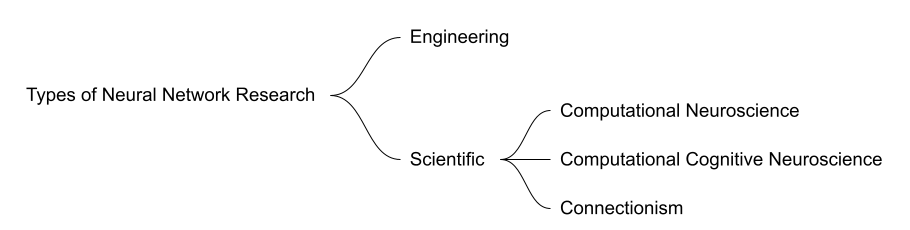
\includegraphics[scale=0.4]{./images/TypesOfNNResearch.png}
\caption[Jeff Yoshimi.]{A taxonomy of types of neural network research, which serves as a guide to this section. Engineering uses (section \ref{machineLearning}) where the goal is to just make something useful, and scientific models where the goal is use neural networks to model the mind (connectionism, section \ref{connectionism}), the brain (computational neuroscience, section \ref{computationalNeuroscience}), or both (computational cognitive neuroscience, section \ref{mixedCases}).}
\label{typesNN}
\end{figure}

Neural networks used for scientific modeling subdivides into several subcategories, depending on what specifically is being simulated. Neural networks are sometimes used to understand the brain (in the field of ``computational neuroscience''), sometimes to understand mind and behavior (this is sometimes called ``connectionism''), and sometimes to understand both brain and mind simultaneously. A map of these types of research is in figure \ref{typesNN}. As we will see, this taxonomy is not always so neat, and there are fascinating cases of, for example, engineering neural networks becoming objects of scientific interest.

A good rule of thumb when considering how to classify a neural network model is to ask: ``What is the neural network being used for? As a tool that does something useful, or as a scientific model?''\footnote{A more advanced way to ask this question is to ask: how are the node activations and weight strengths being interpreted? Are they merely parameters in statistical models, or are they supposed to capture something real about neurons, or about concepts and their relations?} Even then it can be tricky. For example, consider the following title of a journal article: ``Use of Neural Networks in Brain SPECT to Diagnose Alzheimer's Disease'' \cite{page1996use}. At first, this sounds like it might be scientific model, since it mentions the brain and Alzheimer's. However, the article is actually about how neural networks can be used to determine whether a person has Alzheimer's. The neural network is not being used as a model of the brain or any cognitive processes, but rather as an engineering tool to help diagnose Alzheimer's disease based on brain images. If we ask: ``What is the neural network they made being used for?'', the answer is to build a better diagnostic tool for Alzheimers. The network is \emph{not} being used a model of Alzheimers. So it's really an engineering usage of a neural network, rather than a scientific model.

\section{Engineering uses of neural networks}\label{machineLearning}

% Other engineering uses: 
% Fausett section 1.3
% Wiki deep  learning page

Neural networks in engineering are tools to solve problems. They are used as classifiers, controllers, signal processors and other components, alongside many other types of engineering tools. In fact, in the contemporary world, many things we take for granted are built on top of neural networks engineered to do useful things. They are at the heart of the current revolution in AI (as of 2023). They recognize voice and images, they generate speech, the generate images and movies, they drive cars, and of course, they can have human-like conversations with us (as with large language models like ChatGPT). They do many of the things humans do, often better than we can, because we can carefully engineer them and train them on such massive datasets.

We will see in later chapters how to systematically classify these different kinds of models, but for now we can focus on a very common case: the use of neural networks to classify objects, which is  one application of  \glossary{machine learning}. Classifiers are good at  finding patterns in complex and noisy data. Remember, neural networks are trained, not programmed, making them well suited to tasks where there is no obvious way to mathematically determine the relationship between a set of inputs and a set of outputs.

% As two workers in the field put it:
%\begin{quote}
%The most natural application areas for [neural networks] are obviously tasks in which appropriate transformations from certain inputs to certain outputs should be established, but the transformations cannot be discovered analytically due to a variety of reasons. Therefore it is no wonder that the most successful applications of the [neural networks] can be found in the areas of machine vision, pattern recognition, motor control, signal processing, etc., where such input to output transformations dominate the problem solving \cite{heikkonen1999building}.
%\end{quote}
%Engineers who use neural networks for these purposes don't care about how the brain works or how humans think: they want to make a machine that works. A neural-network based rice cooker (like the ``Zojirushi neuro-fuzzy rice cooker''; google it!) should make good rice, whether it cooks like humans do or not. 

\begin{figure}[h]
\centering
\raisebox{-0.5\height}{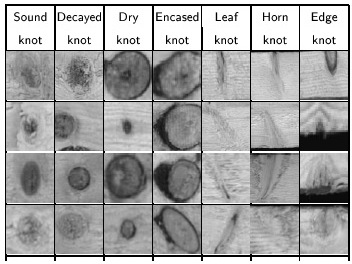
\includegraphics[scale=.4]{./images/wood_network_stimuli.jpg}}
\hspace*{.2in}
\raisebox{-0.5\height}{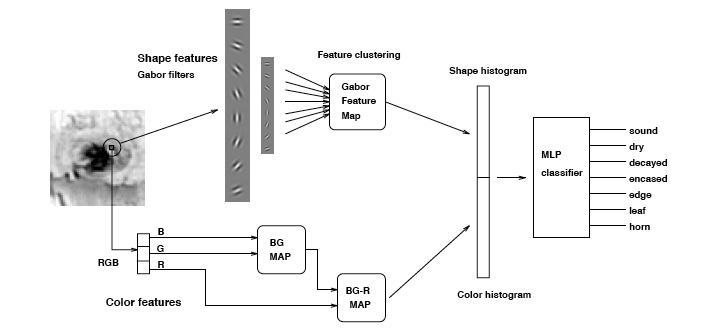
\includegraphics[scale=.3]{./images/wood_network_flowchart.jpg}}
\caption[From Heikkonen et al., 1999 \cite{heikkonen1999building}. Licensed Under CC BY-NC]{Left: Sample inputs to the knot classification network. Right: The knot classification system. The neural network is labelled ``MLP.''}
\label{knotNet}
\end{figure}

Here is an example from the late 1990s. A lumber yard in Finland had to classify pieces of wood, identifying 30 different kinds of knot in images of lumber. Some examples are shown on the left side of figure \ref{knotNet}. A human can classify these knots, but it is time-consuming, expensive, and error-prone (look at how subtle some of the differences are between the different ``dry knots''). It is also hard to program a computer to classify these knots according to explicit rules. Thus, neural networks were used, and they outperformed humans. A neural network trained on samples like the one shown have about 90\% accuracy in this process, compared with 70-80\% accuracy for humans. The neural network is shown in the figure. It is  buried inside the system, the ``MLP classifier'' towards the right (``MLP'' means ``multi-layer-perceptron,'' which is a feed-forward network trained by backpropogation. It is  similar to the 3-object detector above). This system takes a picture of a piece of wood, does some pre-processing on the resulting pixel image, and then summarizes features and colors of that image as a list of numbers, which is fed to the neural network as input. The neural network transforms these numbers into another list of numbers, which describe how decayed, burnt, dry, round, and so forth each sample is. This is a \emph{feature vector}. This feature vector can then be used to classify the knot \cite{heikkonen1999building}.\footnote{Pre-processing is one aspect of data wrangling, which is discussed in chapter \extref{ch_data_science}.  Post-processing also occurs, for example all things that happen in ChatGPT  after the network produces its raw output (for example filtering out inappropriate responses).}
% TODO: Here or above in environment? why here? And make clear processing -> vector -> vector -> post-processing

\section{Computational neuroscience}\label{computationalNeuroscience}

We now turn from neural networks used as engineering tools, to neural networks used as models of the mind and brain.

\glossary{Computational neuroscience} uses computational methods to answer questions related to neuroscience. Computational neuroscience spans many levels, from the micro-scale of cell membranes to the macro-scale of the human brain as a whole (see Fig. \ref{compNeuro}). It is a highly multidisciplinary field, encompassing biology, neuroscience, psychopharmacology, cognitive science, complexity science, psychology, and even physics, depending on the context. 

\begin{figure}[h]
\centering
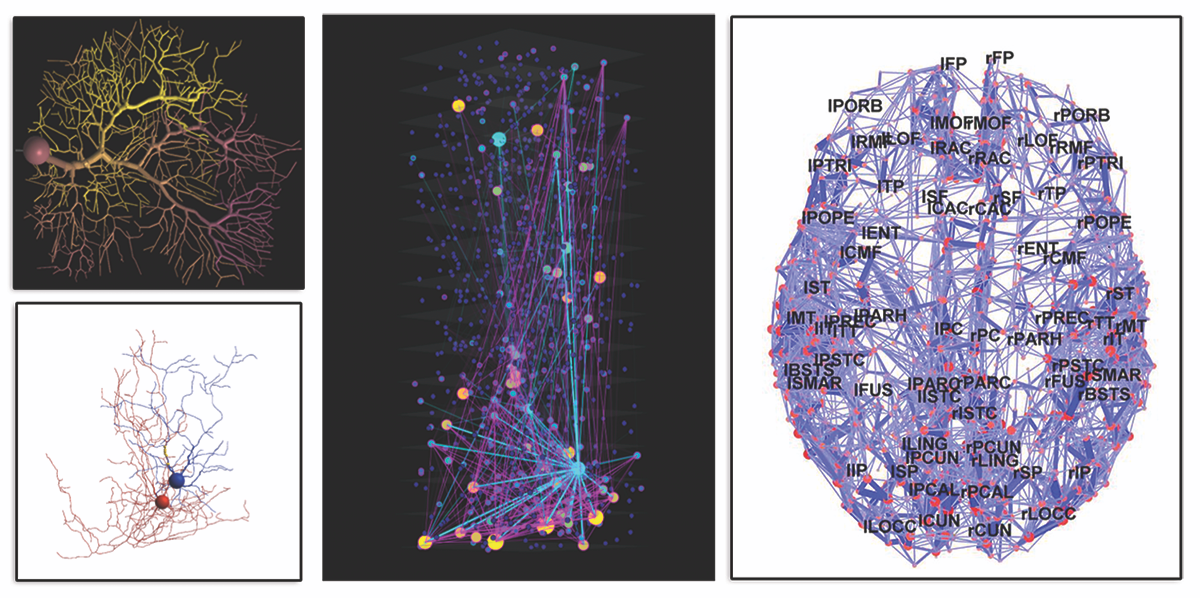
\includegraphics[width=0.8\textwidth]{./images/3typesmodels.png}
\caption[Layout by Pamela Payne. Top Left: ; Bottom Left: ; Middle: Screenshot by Zach Tosi ; Right: From Hagmann et al., 2008 \cite{hagmann2008mapping}, Licensed Under CC BY]{Micro, meso, and macro-level models in computational neuroscience. Left: micro-level models of individual neurons. Middle: meso-level model of a network of several thousand neurons. Right: macro-level model of neuronal connections spread out through the entire brain.}
\label{compNeuro}
\end{figure}
% http://medicalxpress.com/news/2013-11-entire-brain-brainbow-ii-technology.html
% https://upload.wikimedia.org/wikipedia/commons/thumb/e/ef/Network_representation_of_brain_connectivity.JPG/1280px-Network_representation_of_brain_connectivity.JPG

\emph{Micro-scale} models in computational neuroscience study individual neurons or even individual parts of neurons, like the receptors that are studded in the cell membrane to let charged particles in and out of a cell (these are models of ``receptor kinetics''). Models at this level often study the details of how charge flows through the tree-like structures of a neuron's dendrites and axons, and can accurately describe the behavior of individual neurons in a laboratory dish (``in vitro'') when they are injected with current from small electrodes. Models at this level often attempt to answer questions that are physiological or pharmacological in nature like the effect of neuromodulators on the low level dynamics of a neuron, or how new receptors are created or new dendritic spines are grown. These models are largely below the level of what is visible in a single Simbrain node.

\emph{Macro-scale} models in computational neuroscience describe the behavior of large groups of thousands to millions of neurons  and the connections between them. Oftentimes these models approximate the activity of thousands of neurons or even whole brain areas as the activity of a single higher level node.\footnote{As an example, see \url{https://www.ncbi.nlm.nih.gov/pubmed/21511044} \cite{cabral2011role}} These models can accurately describe the spatio-temporal organization of patterns of neural activity measured using brain imaging techniques like fMRI. In a Simbrain network simulation of this kind each node would represent the aggregate activity of thousands to millions of neurons and the whole network could represent the behavior of the entire brain. Models of this type are usually concerned with questions which are psychological or behavioral in nature. For instance the functional relationships between brain regions have been shown to be different in patients with schizophrenia resulting in a different overall graph structure of the functional connectivity between brain regions \cite{bullmore2009complex}. Often work at this level ``bleeds over'' into the realm of general neuroscience.

In this book we mostly focus on the \emph{meso-scale} (or ``middle''-scale) of computational neuroscience, between the micro and macro-levels. Whereas micro-scale models focus on individual neurons or their parts, meso-scale models focus on networks of \emph{hundreds to thousands} (or more) of interconnected neurons. And whereas each node in a macro-level model \emph{approximates} the activity of large group of real neurons, each of the simulated neurons in a meso-level simulation  corresponds to a real neuron. Thus, a meso-level simulation containing 1000 artificial neurons is a direct simulation of a biological neural network containing 1000 real neurons. The emphasis is on discerning governing principles and dynamical phenomena associated with these networks. Meso-level models in computational neuroscience have been implemented in Simbrain (e.g. the middle image in Fig. \ref{compNeuro}). 

The model neurons and synapses used in these simulations  are  more complex than the simple nodes and weights described above in Sect. \ref{structureNets},  since they are designed to mimic the electrochemical properties of real nerve cells. Most neuron models in computational neuroscience are governed by equations acting on variables which represent specific electrochemical attributes of living neurons. Synapses have temporal delays and their signals have duration. Network models in computational neuroscience tend to be comprised of \emph{spiking neurons} (neuron models which produce and propagate signals via action potentials) embedded in complex \emph{recurrent} networks. We cover the special properties of these model neurons and networks in chapter \extref{ch_spiking}.\footnote{In contrast to the micro-scale, which is (broadly) concerned with physiology, and the macro scale, which is often concerned with psychology, the meso-scale concerns itself with questions like: How do networks of interconnected neurons represent information? Can we replicate synaptic connectivity using plasticity rules? How does information processing emerge from the interactions of neurons embedded in a neural network?'  Meso-scale models often attempt to understand formalisms that describe observations of groups of neurons (e.g. slices of brain tissue) with explanations of those observations using models of detailed low level processes at the micro-scale. It is known that when neurons fire in particular temporal sequences the synapses connecting them will become stronger or weaker depending upon that sequence. A micro-scale model might concern itself with how new receptors are created, or new spines are grown. A meso-scale model will only concern itself with the function translating that temporal sequence into a change in synaptic strength.} 

Very roughly, the focus of computational neuroscience at these  three scales can be thought of as follows:
Neuron Dynamics $\rightarrow$ Network Dynamics $\rightarrow$ Brain Dynamics

\section{Connectionism}\label{connectionism}

% Need a footnote or paragraph just surveying a lot of the work in this area.  Also put in another link to this table with papers involving lesions and ablation studies of neural networks: \url{https://link.springer.com/article/10.1007/s42113-020-00081-z/tables/1}

% I think Smolensky's PTC is the best overall discussion.  While the level of analysis adopted by most connectionist cognitive models is not the conceptual [symbolic] one, it is also not the neural level." See the discussion surrounding 7.  Then can refer back to this in history and in intro symbolic vs. parallel. Nice distinction between activation evolution equation and connection evolution equation.

% See Talking Nets 259, 283, 274
% Maybe talk more about semantic memory and semantic network models, and contrast with other types of memory (many will not have taken intro cog-sci courses)
The use of neural networks as cognitive models, which behave in the same way humans and animals do, but without concern for neural realism, is sometimes called \glossary{connectionism}.\footnote{Not everyone using the term ``connectionism'' in this way, but it is a fairly standard usage. A more precise phrase would be ``connectionist model of a cognitive process''.}  In connectionist models, there is no direct effort to understand the brain. The focus is on modeling some aspect of human or animal behavior using nodes and weights. Such models  are usually meant to {\em suggest} how a given task is accomplished by the brain---they are ``neurally plausible''---but they do not directly model the underlying neuroscience.

% Should this be a named section on IAC? Kind of lost in this organization.
% Redo IAC given assignments
% Forward reference to ch_unsupervised_recurrent and DST, it develops fixed point attractors and the transient portion is the thought process
% We have settled on object pool and property pool. Introduce this nomenclature and distinguish it from the original.  Also, use some memory language. Item vs. category retrieval. "exemplars. It can also generalize along an indefinite number of different lines retrieve the specific characteristics of particular exemplars , and fill in plauaible default values for misaing properties."
As an example, consider the ``IAC'' or ``Interactive Activation and Competition'' network. A famous example of an IAC network is McClelland's model of knowledge of two fictional 1950s gangs, the Jets and Sharks from {\em West Side Story} \cite{mcclelland1981retrieving}.\footnote{For a video overview of this network in Simbrain, see \url{https://www.youtube.com/watch?v=Nw3TEDfugLs}.}

\begin{figure}[h]
\centering
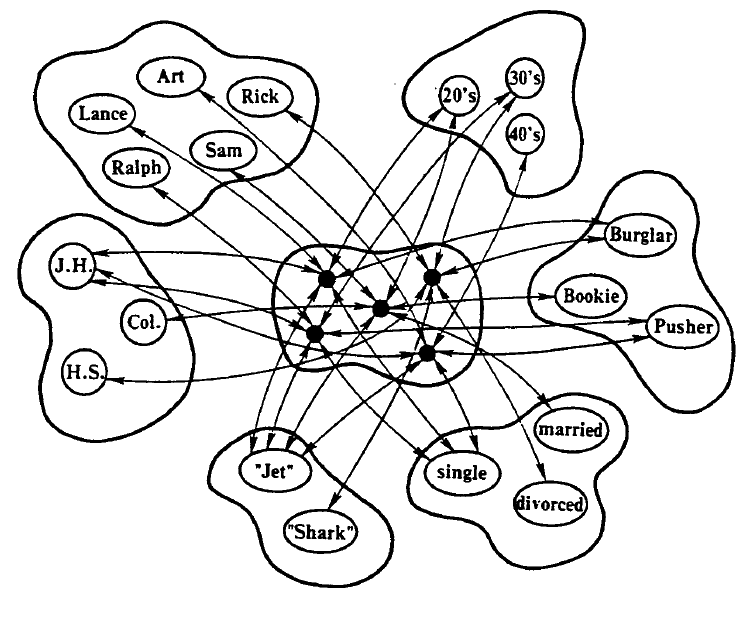
\includegraphics[scale=.3]{./images/IAC_JetsSharks.png}
\caption[From McClelland and Rumelhart, 1989 \cite{mcclelland1989explorations}.]{A fragment of the Jets and Sharks model. Nodes in this model don't represent neural activity, but activation of concepts in semantic memory.}
\label{iac}
\end{figure}

% Maybe just go full Simbrain. Change the example and make clear that it can be done in many ways.

% In a sense a model of the ventral stream, but not the dorsal stream. No ``embodied'' memory captured, no dorsal stream, and no retrieval mechanisms. Maybe refer to publications about actual semantic memory. BUT don't want to emphasize neuro too much so a balance.
% A good contrast to supervised, unsupervised, and generalization. A strange case where we hand-tune the weights. Note there is NO learning in these model. So the concepts of supervised and unsupervised don't apply. It is hand tuned. 

% Make the object pool / property pool distinction more central, and give more examples. There is no rock solid way to define object vs property philosophically, but functionally there are things we're talking about, and then there are our beliefs about their properties and characteristics.  The objects is like a thing that is a locus of these believes so they are in the center.  In IAC it's the people but it could also be teams, games, etc. (philosophers would wince, because object pools can even be properties)! Whatever is central is the object nodes,  // Also note that we stopped making separate name and object nodes. Maybe we could just call them name nodes.

An IAC model is organized into pools of nodes. In Fig. \ref{iac}, there are 7 pools of nodes. These pools of nodes are used to model the internal concepts of a person who knows about these two gangs. The pools represent different  traits:  age, education level, marital status,  job, etc. The central pool is a pool of ``instance nodes'' or ``object nodes'', shown as black disks, which correspond to individual people. Each person is associated with a node. The other pools correspond to properties of these people: their name, job, age, and gang affiliation. The nodes in each pool inhibit each other, which produces a \emph{winner-take-all} structure. As the simulation runs, the activation of one node in each pool will tend to dominate the others. Notice that the topology of this network is recurrent, and as a result the network has dynamics: when we run it, activation starts to spread from one node to another over time. In fact, these have also been called \emph{spreading activation} networks \cite{mcclelland1981retrieving}. 

The IAC network models general features of human semantic memory, like the ability to retrieve attributes of a person based on their name. If the Lance node is activated and the simulation is run, activation will spread through the recurrent network, and after a while the Jets node, 20s node, Junior high education node, and burglar node will have the highest activations. This is like asking ``Tell me about Lance?'' and being told about him. The network can also model our ability to describe the properties of a group of people. If the Jets node is activated and the network is run, the standard characteristics of the Jets will light up: they tend to be in their 20s, with a junior high school education, and single. This is like asking ``Tell me about the Jets?'' and being told about that group. The network can also model our ability to identify people who match a specific description. If the 20s node and the junior-high education node are activated, then the name nodes for Lance, Jim, John, and George all light up. This is like asking ``Who is in their 20s with a junior high education?'' and being told ``Well, that could be Lance, Jim, John, or George.''
%\footnote{Notice that the nodes and connections in this model don't correspond to actual neurons or synapses. The IAC network captures the empiricist theory (associated with John Locke and David Hume) that  human knowledge is encoded in abstract associations between ideas. Node activations correspond to the presence of an item in thought or memory, or what the empiricist philosophers called \emph{ideas}. If the ``Lance'' node is active, that corresponds to a person thinking about Lance. Connections between nodes correspond to \emph{associations} between ideas. The whole network of connections represents our overall knowledge about something, in this case, two gangs. When one node  is activated and the network is run, all the associated nodes are activated. Over time all the ideas associated with the original idea should be activated \cite{mcclelland1981retrieving}. Nodes and weights represent ideas and associations in an abstract brain-like way without modeling neuroscience directly.} \cite{mcclelland1981retrieving}

Though IAC networks are models of semantic memory, and are brain-like (spreading activation and winner-take-all types of dynamics do occur in the brain), they are \emph{not} models of the brain, they do not capture any details of human neuroscience, or have nodes whose activation corresponds to activity in specific parts of the brain.

\begin{figure}[h]
\centering
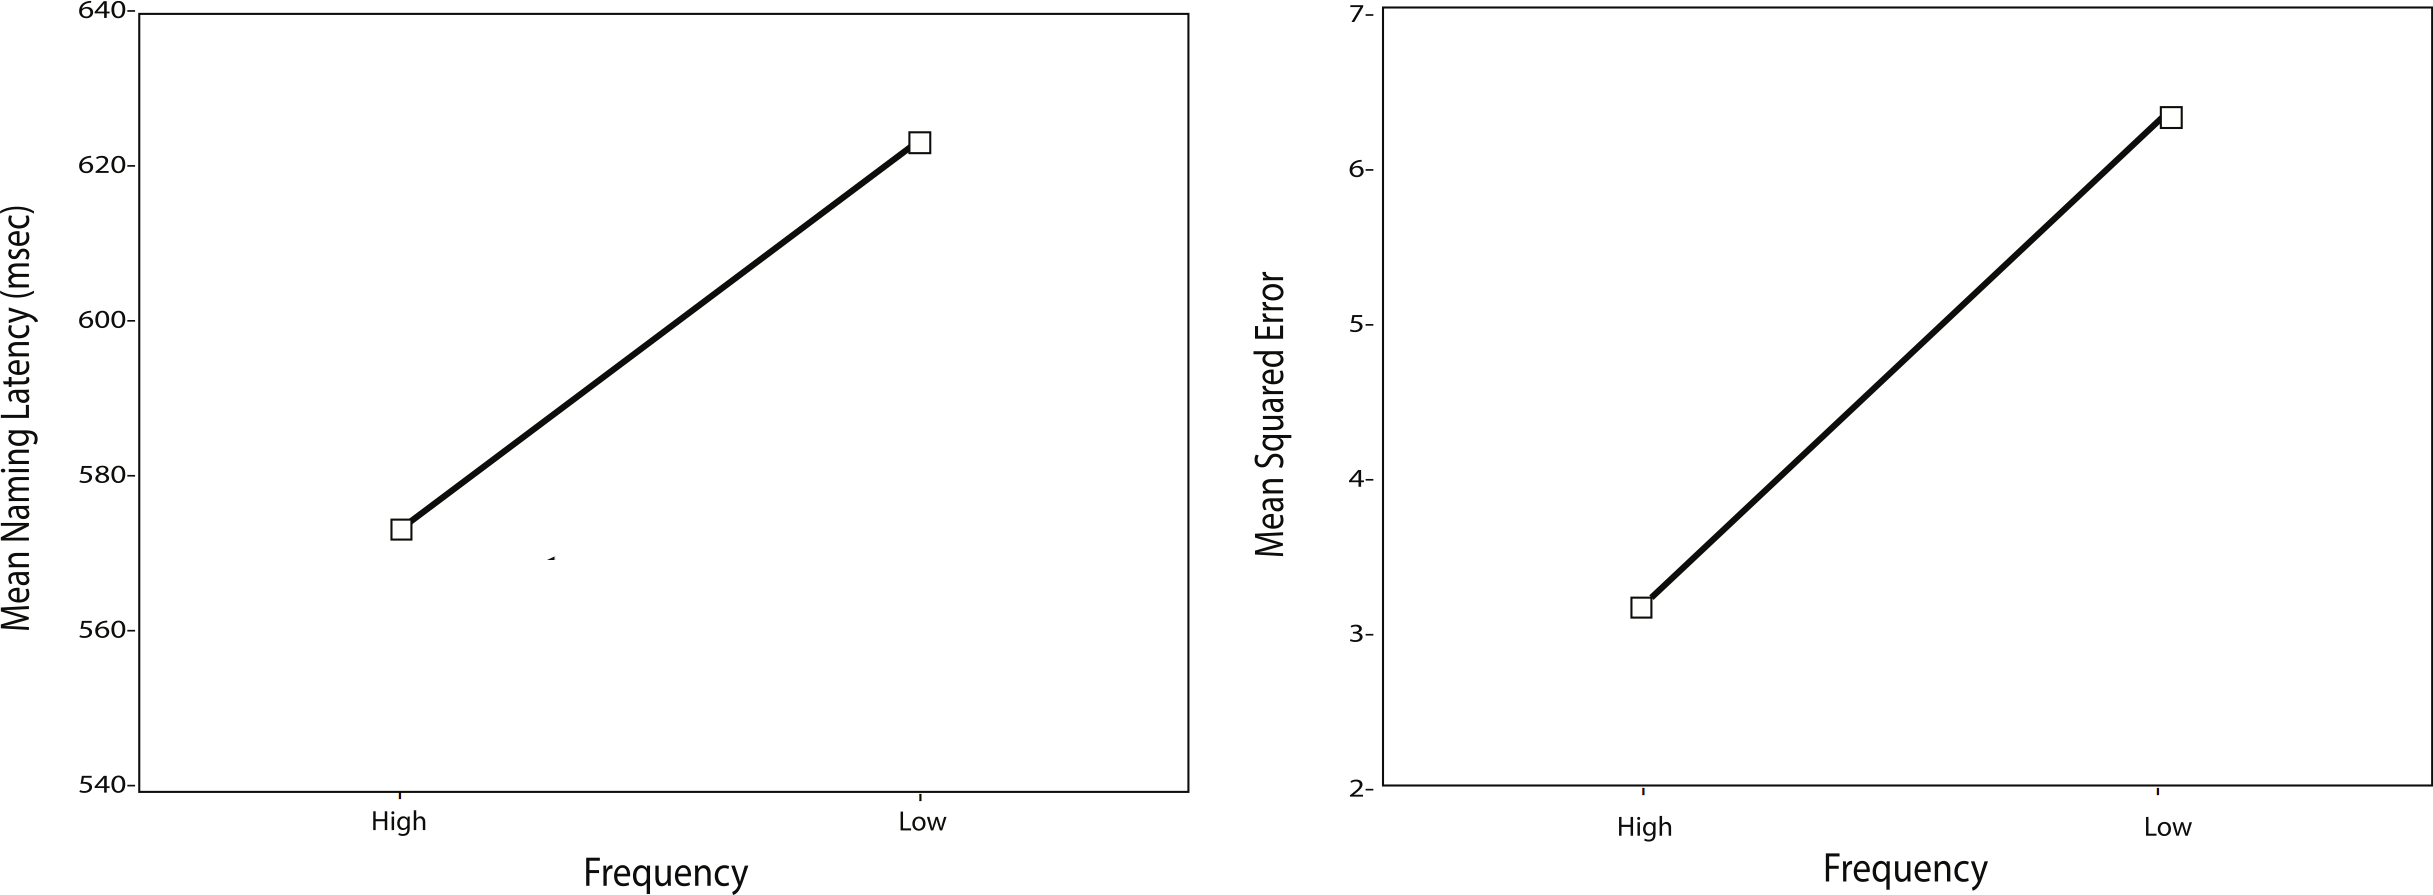
\includegraphics[width=0.8\textwidth]{./images/seidWordNet_Data3.png}
\caption[From McClelland and Seidenberg, 1989 \cite{seidenberg1989distributed}. Redrawn by Pamela Payne.]{Data associated with Seidenberg and McClelland (1989)'s reading model. Human data are on the left, neural network data are on the right. Humans pronounce high-frequency words more quickly than low-frequency words. The neural network makes fewer errors on high-frequency than low-frequency words.}
\label{regularityData}
\end{figure}
 
% This has become so short it might be time to get remove it, keep things simple. One main example per section. As it is it gets a bit lost. If used, take the opportunity to talk about error in a bit more detail.
The IAC network is a qualitative model of human memory. Other connectionist simulations are more quantitative. For example, Seidenberg and McClelland modeled childrens' reaction times in reading words aloud. The network is a variant on a feed-forward network, similar to the network on the left side of figure \ref{nn_types}. It has  more nodes: 400 input units, which represent written words, and 460 output units, which represent spoken words. It was trained to pronounce all one-syllable words in English using a method called ``backpropogation'' (chapter \extref{ch_supervised}). This simulation models  the \emph{word-frequency effect}. Words that occur frequently in language (like ``the'') are pronounced more quickly than words that occur infrequently (like ``rake'').
%\footnote{\label{exceptionsVsRegular}The model also captures the ``frequency-regularity interaction'', whereby words that have regular pronunciation patterns (e.g. ``gave'' or ``must''), are pronounced faster than exception words (e.g. ``have''  or ``pint''). However, this regularity effect only occurs for infrequent words. This is also shown in the figure: in each graph the upper curve with the open squares show exception words; the lower curves with filled triangles show regular words.}  

Human data showing this effect are on the left side of Fig. \ref{regularityData}. Humans pronounce high-frequency words more quickly than low-frequency words (the $y$-axis shows latency, or length of time to pronounce the word; lower values mean faster times). The neural network data on the right  was generated by counting how many mistakes the network made for low and high frequency words \cite{seidenberg1989distributed}. When you line the two graphs up next to each other, they look the same. This suggests that the way the model reads is similar to the way humans read: both the neural network model and humans are better at reading more common words.
%\footnote{ Many questions come up here, and you might not be satisfied (in fact, this model was involved in a kind of war between connectionist and non-connectionist models of  reading). The main thing  to emphasize here is that the model is supposed to capture some kind of human, behavioral data.}

\section{Computational Cognitive Neuroscience}\label{mixedCases}

 For neural network used as scientific models, it can be hard to say whether it simulates the brain (computational neuroscience), or cognition (connectionism). Many models aim to do both at once.
That is, many people who use neural network models are interested in \emph{both} how the brain works \emph{and} how cognition works, and of course, how the two are related. Thus, there are increasingly many models that attempt to capture both neural and psychological data, as was noted in the discussion of macro-level computational neuroscience above. 

We will refer to these as \glossary{computational cognitive neuroscience} models, and define them as models that attempt to capture psychological and behavioral data while simultaneously paying attention to neural details. This type of model captures various aspects of cognition (e.g. visual attention, semantic and episodic memory, priming, familiarity, and cognitive control), using groups of neurons that are explicitly associated with specific brain circuits. Many researchers hope that over time computer models of brain and behavior will converge, and that future models will increasingly capture both neural and behavioral data, and thereby reveal how the dynamics of the brain give rise to the dynamics of cognition.\footnote{Examples of researchers and research groups working in this area include the work of Randy O'Reilly and his colleagues (\url{https://grey.colorado.edu/CompCogNeuro/index.php/CCNBook/Main}), Stephen Grossberg's work which began in the 1960s (\url{https://en.wikipedia.org/wiki/Stephen_Grossberg}), and the work of Chris Eliasmith and his colleagues (\url{https://uwaterloo.ca/centre-for-theoretical-neuroscience/people-profiles/chris-eliasmith}). There is also a burgeoning research community organized around the computational cognitive neuroscience conference (here is their 2024 program: \url{https://2024.ccneuro.org/}).} Some examples of this type of model are shown in figure \ref{ccn}.

% Emergent ref since I have a spaun ref?
\begin{figure}[h]
\centering
\raisebox{-0.5\height}{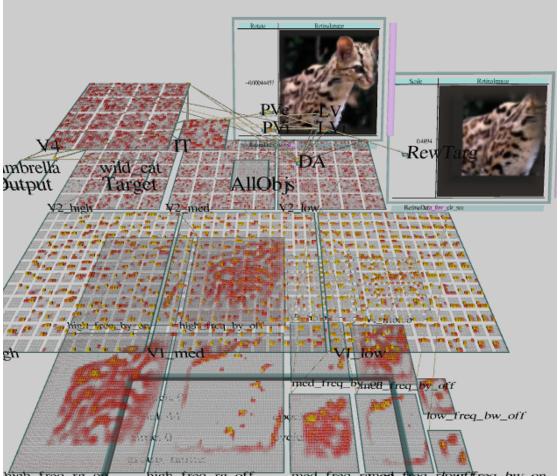
\includegraphics[scale=.3]{./images/EmergentScreenshot.png}}
\hspace*{.4in}
\raisebox{-0.5\height}{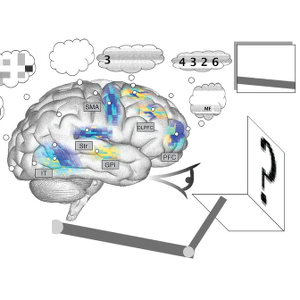
\includegraphics[scale=.6]{./images/spaun.png}}
\caption[Left: From \url{https://grey.colorado.edu/emergent/index.php/File:Screenshot_vision.png}; Right: Spaun screenshot. Cf. \cite{eliasmith2012large}.]{(Left) An Emergent simulation of visual processing, with labels indicating which brain areas each group of nodes represents. (Right) A Nengo simulation of the human ability to retrace a visually perceived number.}
\label{ccn}
\end{figure}

 From this standpoint, computational neuroscience and connectionism are two ends of a continuum or spectrum. We have computational neuroscience at one end, and connectionism at the other. All through the middle of this spectrum are models that try to model both biological data and psychological data at the same time. The goal is to understand how the circuits of the brain produce all the wealth and complexity of observable human and animal behavior. 

\section{From science to engineering and from engineering to science}

Some neural networks that originated as scientific models later informed the development of engineering tools. Conversely, sometimes an engineering tool ends up being useful as a scientific model. These are interesting historical dynamics.
 
 Deep networks provide a good example of these back and forths. Deep neural networks  were originally used as scientific models of vision in the 1970s (see chapters \extref{ch_history} and  \extref{ch_neuro}).  These early neural network models of vision turned out to be excellent tools for pattern recognition, a common engineering application, for example recognizing digits on an envelope. This is part of what led to the deep learning revolution of the 2010s. So we had a shift from science to engineering. But then it happened again, in the reverse direction. These new and improved deep networks turned out to be useful in computational neuroscience as a way to understand the human visual system. So, a neural network that started off in science, then got used for engineering, and then that tool later got adapted back to science! 

Similar twists and turns from engineering to science are happening now with the emergence of large language models like ChatGPT. They originated as pure engineering models, that are meant to facilitate natural language processing. I think we can all agree that ChatGPT is useful, whether or not it ``thinks like a human.'' But it's so compelling as a model, that linguists, psychologists, and philosophers now routinely study them as cognitive models. See section \extref{llm_cogsci}. So in this case a model that started off in engineering subsequently also became an object of scientific study. 

%In fact, a whole area of study--``mechanistic interpretability'' (see chapter \extref{ch_mechinterp})--has emerged whose aim is to understand how these neural networks work internally: 
 
